\documentclass[11pt]{article}
\usepackage[margin=1in]{geometry}
\usepackage{amsmath,amssymb}
\usepackage{tikz}
\usepackage{pgfplots}
\usepackage{booktabs}
\usepackage{xcolor}

% Brand colors
\definecolor{garnet}{HTML}{73000A}
\definecolor{atlantic}{HTML}{466A9F}
\definecolor{congaree}{HTML}{1F414D}
\definecolor{horseshoe}{HTML}{65780B}
\definecolor{rose}{HTML}{CC2E40}
\definecolor{black90}{HTML}{363636}
\definecolor{black70}{HTML}{5C5C5C}

\pgfplotsset{compat=1.18}

% Unit commands
\newcommand{\degC}{$^\circ$C}
\newcommand{\unit}[1]{\,\mathrm{#1}}

\title{\textbf{Heat Transfer Through Air Between a Hot Source and Cold Wall}}
\author{J.C. Vaught}
\date{\today}

\begin{document}
\maketitle

\section{Problem Statement}

Consider heat transfer through an air gap between a hot surface at $T_h = 90$\degC{} and a cold wall at $T_c = 20$\degC{}. The air gap has thickness $L = 0.05\unit{m}$ and cross-sectional area $A = 1\unit{m^2}$. We analyze two cases:
\begin{enumerate}
    \item \textbf{Stagnant air} -- heat transfer by conduction and natural convection
    \item \textbf{Moving air} -- heat transfer by forced convection
\end{enumerate}

\section{System Diagram}

\begin{figure}[h]
\centering
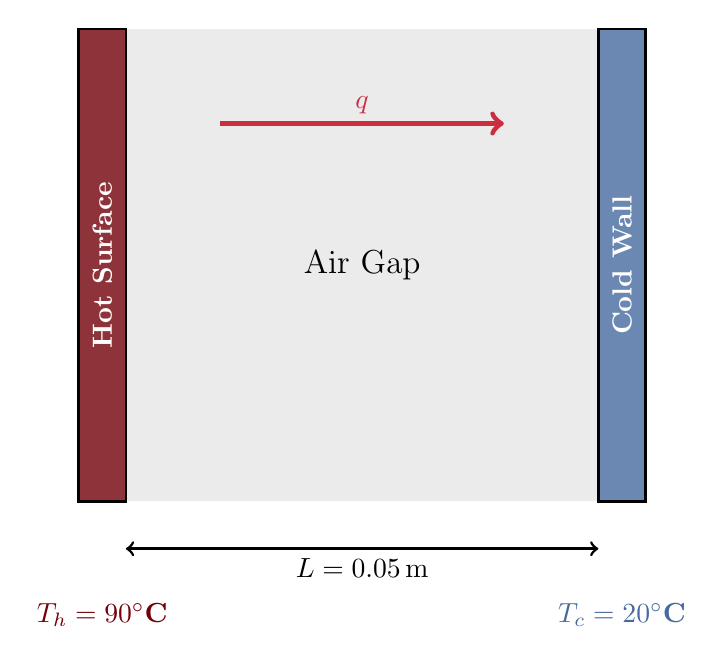
\begin{tikzpicture}[scale=1.2]
    % Hot wall
    \fill[garnet!80] (0,0) rectangle (0.5,5);
    \draw[line width=1pt] (0,0) rectangle (0.5,5);
    \node[rotate=90, white, font=\bfseries] at (0.25,2.5) {Hot Surface};

    % Cold wall
    \fill[atlantic!80] (5.5,0) rectangle (6,5);
    \draw[line width=1pt] (5.5,0) rectangle (6,5);
    \node[rotate=90, white, font=\bfseries] at (5.75,2.5) {Cold Wall};

    % Air gap
    \fill[black90!10] (0.5,0) rectangle (5.5,5);
    \draw[line width=1pt] (0.5,0) -- (0.5,5);
    \draw[line width=1pt] (5.5,0) -- (5.5,5);

    % Air label
    \node[font=\large] at (3,2.5) {Air Gap};

    % Dimensions
    \draw[<->, line width=1pt] (0.5,-0.5) -- (5.5,-0.5);
    \node[below] at (3,-0.5) {$L = 0.05\unit{m}$};

    % Temperatures
    \node[garnet, font=\bfseries] at (0.25,-1.2) {$T_h = 90$\degC};
    \node[atlantic, font=\bfseries] at (5.75,-1.2) {$T_c = 20$\degC};

    % Heat flow arrow
    \draw[->, line width=2pt, rose] (1.5,4) -- (4.5,4);
    \node[above, rose, font=\bfseries] at (3,4) {$q$};
\end{tikzpicture}
\caption{Schematic of heat transfer through an air gap between hot and cold surfaces.}
\label{fig:schematic}
\end{figure}

\section{Air Properties}

We evaluate air properties at the film temperature:
\begin{equation}
    T_f = \frac{T_h + T_c}{2} = \frac{90 + 20}{2} = 55\text{\degC} = 328\unit{K}
\end{equation}

\begin{table}[h]
\centering
\caption{Air properties at $T_f = 55$\degC}
\begin{tabular}{lll}
\toprule
\textbf{Property} & \textbf{Symbol} & \textbf{Value} \\
\midrule
Thermal conductivity & $k$ & $0.0283\unit{W/(m \cdot K)}$ \\
Density & $\rho$ & $1.076\unit{kg/m^3}$ \\
Dynamic viscosity & $\mu$ & $1.96 \times 10^{-5}\unit{Pa \cdot s}$ \\
Kinematic viscosity & $\nu$ & $1.82 \times 10^{-5}\unit{m^2/s}$ \\
Specific heat & $c_p$ & $1007\unit{J/(kg \cdot K)}$ \\
Thermal diffusivity & $\alpha$ & $2.59 \times 10^{-5}\unit{m^2/s}$ \\
Prandtl number & $Pr$ & 0.703 \\
Thermal expansion coeff. & $\beta$ & $3.05 \times 10^{-3}\unit{K^{-1}}$ \\
\bottomrule
\end{tabular}
\label{tab:properties}
\end{table}

\section{Case 1: Stagnant Air (Natural Convection)}

\subsection{Pure Conduction (Lower Bound)}

If no convection occurs, heat transfers only by conduction:
\begin{equation}
    q_{cond} = \frac{kA(T_h - T_c)}{L} = \frac{0.0283 \times 1 \times (90 - 20)}{0.05} = \boxed{39.6\unit{W}}
\end{equation}

\subsection{Natural Convection in Enclosure}

For a vertical enclosure, we first calculate the Rayleigh number:
\begin{equation}
    Ra_L = \frac{g\beta(T_h - T_c)L^3}{\nu\alpha}
\end{equation}
\begin{equation}
    Ra_L = \frac{9.81 \times 3.05 \times 10^{-3} \times 70 \times (0.05)^3}{1.82 \times 10^{-5} \times 2.59 \times 10^{-5}} = \boxed{5.58 \times 10^5}
\end{equation}

For a vertical enclosure with aspect ratio $H/L = 20$ (assuming $H = 1\unit{m}$), we use the Berkovsky-Polevikov correlation:
\begin{equation}
    Nu = 0.18 \left(\frac{Pr}{0.2 + Pr} Ra_L\right)^{0.29}
\end{equation}
\begin{equation}
    Nu = 0.18 \left(\frac{0.703}{0.2 + 0.703} \times 5.58 \times 10^5\right)^{0.29} = \boxed{7.42}
\end{equation}

The effective thermal conductivity and heat transfer rate:
\begin{equation}
    k_{eff} = k \cdot Nu = 0.0283 \times 7.42 = 0.210\unit{W/(m \cdot K)}
\end{equation}
\begin{equation}
    q_{nat} = \frac{k_{eff} A (T_h - T_c)}{L} = \frac{0.210 \times 1 \times 70}{0.05} = \boxed{294\unit{W}}
\end{equation}

The convective heat transfer coefficient for natural convection:
\begin{equation}
    h_{nat} = \frac{Nu \cdot k}{L} = \frac{7.42 \times 0.0283}{0.05} = \boxed{4.2\unit{W/(m^2 \cdot K)}}
\end{equation}

\section{Case 2: Moving Air (Forced Convection)}

\subsection{Flow Configuration}

\begin{figure}[h]
\centering
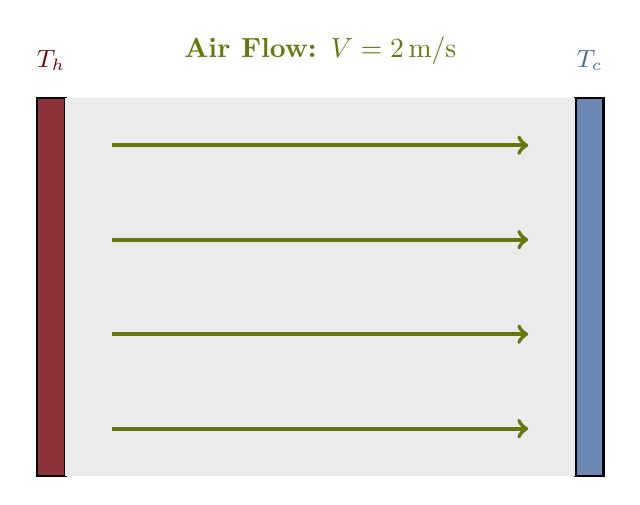
\begin{tikzpicture}[scale=1.2]
    % Hot wall
    \fill[garnet!80] (0,0) rectangle (0.3,4);
    \draw[line width=1pt] (0,0) rectangle (0.3,4);

    % Cold wall
    \fill[atlantic!80] (5.7,0) rectangle (6,4);
    \draw[line width=1pt] (5.7,0) rectangle (6,4);

    % Air gap
    \fill[black90!10] (0.3,0) rectangle (5.7,4);

    % Flow arrows
    \foreach \y in {0.5, 1.5, 2.5, 3.5} {
        \draw[->, line width=1.5pt, horseshoe] (0.8,\y) -- (5.2,\y);
    }

    % Velocity profile hint
    \node[horseshoe, font=\bfseries] at (3,4.5) {Air Flow: $V = 2\unit{m/s}$};

    % Labels
    \node[garnet, font=\small\bfseries] at (0.15,4.4) {$T_h$};
    \node[atlantic, font=\small\bfseries] at (5.85,4.4) {$T_c$};
\end{tikzpicture}
\caption{Forced convection with air flowing through the gap at velocity $V$.}
\label{fig:forced}
\end{figure}

Assume air flows through the gap at velocity $V = 2\unit{m/s}$.

\subsection{Reynolds Number}

Using the gap width as the characteristic length:
\begin{equation}
    Re_L = \frac{\rho V L}{\mu} = \frac{1.076 \times 2 \times 0.05}{1.96 \times 10^{-5}} = \boxed{5490}
\end{equation}

This indicates \textbf{transitional flow} ($Re < 10^5$ for external flow over a plate).

\subsection{Nusselt Number and Heat Transfer Coefficient}

For flow between parallel plates (internal flow, developing), we use:
\begin{equation}
    Nu = 7.54 + \frac{0.03(D_h/L_{flow})Re \cdot Pr}{1 + 0.016[(D_h/L_{flow})Re \cdot Pr]^{2/3}}
\end{equation}

For a simpler estimate using flat plate correlation (laminar):
\begin{equation}
    Nu = 0.664 \, Re_L^{0.5} \, Pr^{1/3} = 0.664 \times (5490)^{0.5} \times (0.703)^{1/3} = \boxed{43.7}
\end{equation}

The forced convection heat transfer coefficient:
\begin{equation}
    h_{forced} = \frac{Nu \cdot k}{L} = \frac{43.7 \times 0.0283}{0.05} = \boxed{24.7\unit{W/(m^2 \cdot K)}}
\end{equation}

Heat transfer rate:
\begin{equation}
    q_{forced} = h_{forced} A (T_h - T_c) = 24.7 \times 1 \times 70 = \boxed{1729\unit{W}}
\end{equation}

\section{Comparison of Results}

\begin{table}[h]
\centering
\caption{Comparison of heat transfer modes}
\begin{tabular}{lccc}
\toprule
\textbf{Mode} & \textbf{$h$ [W/(m$^2$K)]} & \textbf{$q$ [W]} & \textbf{Enhancement} \\
\midrule
Pure Conduction & 0.57 & 39.6 & 1.0$\times$ \\
Natural Convection & 4.2 & 294 & 7.4$\times$ \\
Forced Convection ($V=2$ m/s) & 24.7 & 1729 & 43.7$\times$ \\
\bottomrule
\end{tabular}
\label{tab:comparison}
\end{table}

\section{Parametric Analysis}

\subsection{Heat Transfer vs. Air Gap Thickness}

\begin{figure}[h]
\centering
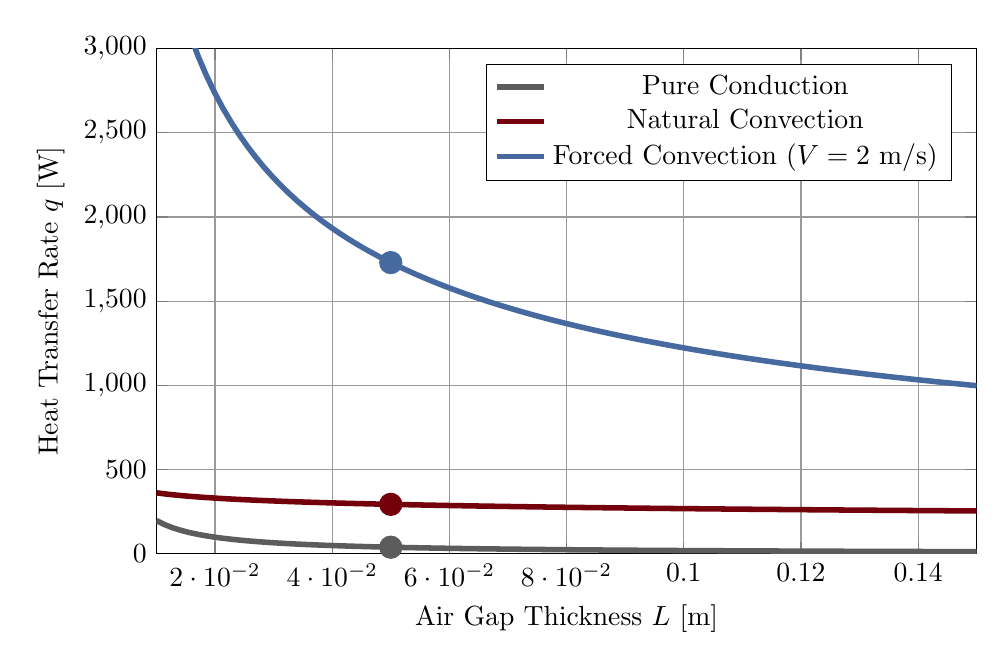
\begin{tikzpicture}
\begin{axis}[
    width=12cm,
    height=8cm,
    xlabel={Air Gap Thickness $L$ [m]},
    ylabel={Heat Transfer Rate $q$ [W]},
    xmin=0.01, xmax=0.15,
    ymin=0, ymax=3000,
    legend pos=north east,
    grid=both,
    grid style={line width=0.2pt, draw=black90!30},
    major grid style={line width=0.4pt, draw=black90!50},
    tick style={line width=0.4pt},
]

% Pure conduction: q = k*A*dT/L = 0.0283*1*70/L = 1.981/L
\addplot[
    domain=0.01:0.15,
    samples=100,
    line width=2pt,
    color=black70,
] {1.981/x};
\addlegendentry{Pure Conduction}

% Natural convection (simplified: Nu scales with Ra^0.29, Ra scales with L^3)
% So Nu ~ L^0.87, h = Nu*k/L ~ L^-0.13, q = h*A*dT ~ L^-0.13
% At L=0.05, q=294, so q = 294*(0.05/x)^0.13
\addplot[
    domain=0.01:0.15,
    samples=100,
    line width=2pt,
    color=garnet,
] {294*(0.05/x)^0.13};
\addlegendentry{Natural Convection}

% Forced convection: Nu ~ Re^0.5 ~ (V*L)^0.5, h = Nu*k/L ~ L^-0.5
% q = h*A*dT ~ L^-0.5
% At L=0.05, q=1729, so q = 1729*(0.05/x)^0.5
\addplot[
    domain=0.01:0.15,
    samples=100,
    line width=2pt,
    color=atlantic,
] {1729*(0.05/x)^0.5};
\addlegendentry{Forced Convection ($V=2$ m/s)}

% Reference point
\addplot[only marks, mark=*, mark size=4pt, color=garnet] coordinates {(0.05, 294)};
\addplot[only marks, mark=*, mark size=4pt, color=atlantic] coordinates {(0.05, 1729)};
\addplot[only marks, mark=*, mark size=4pt, color=black70] coordinates {(0.05, 39.6)};

\end{axis}
\end{tikzpicture}
\caption{Heat transfer rate as a function of air gap thickness for different modes.}
\label{fig:q_vs_L}
\end{figure}

\subsection{Heat Transfer Coefficient vs. Air Velocity (Forced Convection)}

\begin{figure}[h]
\centering
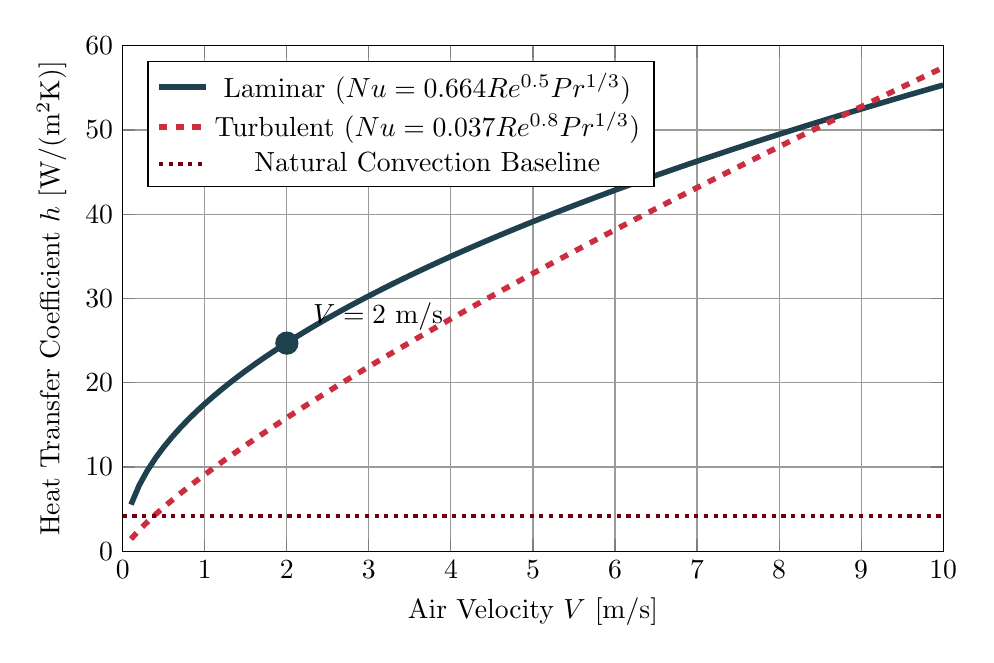
\begin{tikzpicture}
\begin{axis}[
    width=12cm,
    height=8cm,
    xlabel={Air Velocity $V$ [m/s]},
    ylabel={Heat Transfer Coefficient $h$ [W/(m$^2$K)]},
    xmin=0, xmax=10,
    ymin=0, ymax=60,
    legend pos=north west,
    grid=both,
    grid style={line width=0.2pt, draw=black90!30},
    major grid style={line width=0.4pt, draw=black90!50},
    tick style={line width=0.4pt},
]

% h = 0.664 * (rho*V*L/mu)^0.5 * Pr^(1/3) * k / L
% h = 0.664 * (1.076*V*0.05/1.96e-5)^0.5 * 0.703^(1/3) * 0.0283 / 0.05
% h = 0.664 * (2745*V)^0.5 * 0.889 * 0.566
% h = 0.664 * 52.4 * V^0.5 * 0.503 = 17.5 * V^0.5
\addplot[
    domain=0.1:10,
    samples=100,
    line width=2pt,
    color=congaree,
] {17.5*x^0.5};
\addlegendentry{Laminar ($Nu = 0.664 Re^{0.5} Pr^{1/3}$)}

% Turbulent: Nu = 0.037 Re^0.8 Pr^(1/3)
% h = 0.037 * (2745*V)^0.8 * 0.889 * 0.0283 / 0.05
% h = 0.037 * 2745^0.8 * V^0.8 * 0.889 * 0.566 = 0.037 * 489.5 * 0.503 * V^0.8
% h = 9.1 * V^0.8
\addplot[
    domain=0.1:10,
    samples=100,
    line width=2pt,
    color=rose,
    dashed,
] {9.1*x^0.8};
\addlegendentry{Turbulent ($Nu = 0.037 Re^{0.8} Pr^{1/3}$)}

% Natural convection baseline
\addplot[
    domain=0:10,
    samples=2,
    line width=1.5pt,
    color=garnet,
    dotted,
] {4.2};
\addlegendentry{Natural Convection Baseline}

% Reference point
\addplot[only marks, mark=*, mark size=4pt, color=congaree] coordinates {(2, 24.7)};
\node[anchor=south west] at (axis cs:2.2, 25) {$V = 2$ m/s};

\end{axis}
\end{tikzpicture}
\caption{Heat transfer coefficient vs. air velocity for forced convection.}
\label{fig:h_vs_V}
\end{figure}

\section{Conclusions}

\begin{enumerate}
    \item \textbf{Stagnant air} with natural convection provides $\approx 7\times$ enhancement over pure conduction due to buoyancy-driven circulation.

    \item \textbf{Moving air} at $V = 2$ m/s provides $\approx 44\times$ enhancement over pure conduction and $\approx 6\times$ over natural convection.

    \item The heat transfer coefficient scales as:
    \begin{itemize}
        \item Conduction: $h \propto 1/L$
        \item Natural convection: $h \propto L^{-0.13}$ (weak dependence)
        \item Forced convection: $h \propto V^{0.5}$ (laminar) or $h \propto V^{0.8}$ (turbulent)
    \end{itemize}

    \item For maximum heat transfer, forced convection with high velocity and small gap thickness is preferred.
\end{enumerate}

\end{document}
